
\chapter{Family Doodles}

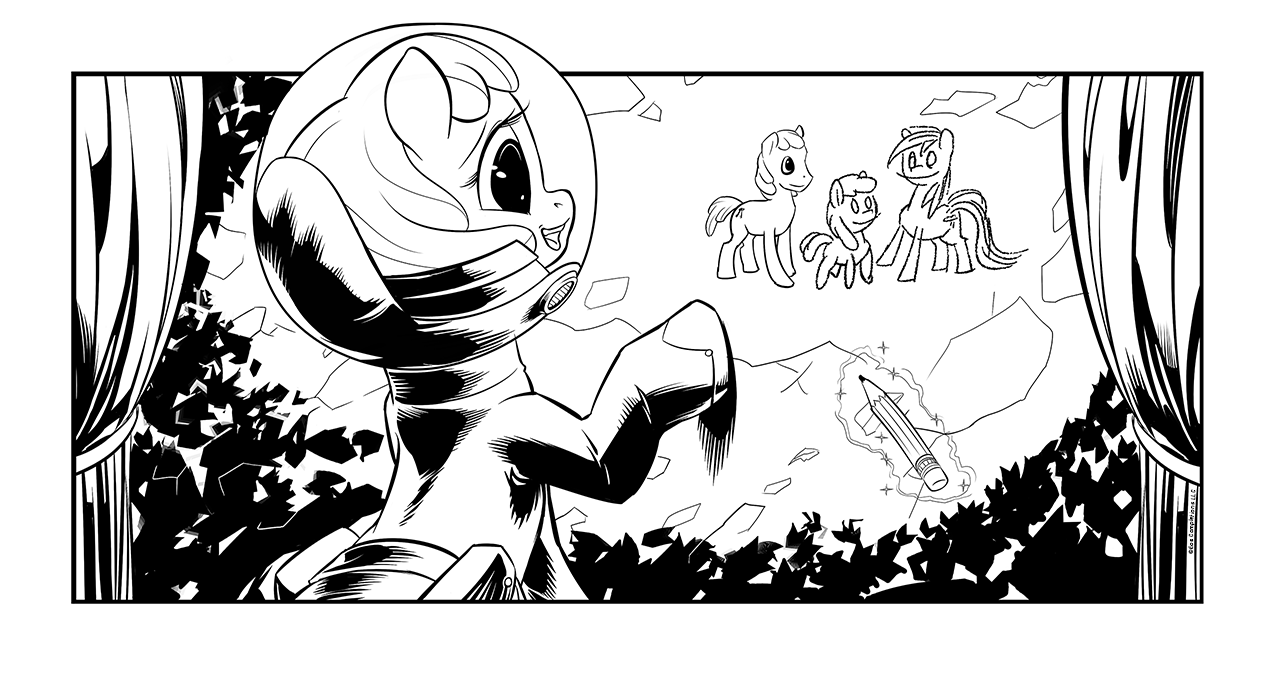
\includegraphics[width=0.9\linewidth]{image11.png}

\begin{intro}
You're not using power tools, are you?
\end{intro}


\englishdaytimeplace{10}{1:30 P.M.}{Rust Manor, Big 52 SC Branch}

\rtpr{Ahem, good afternoon everypony. I am Lonesome Pony, and this is a special edition of the news, fresh from Dust Manor.}

For a moment, the feminine voice of the afternoon DJ could be clearly heard in the background yelling ``Gimme back my seat you hog!'' followed by a metallic sound.

\rtpr{DJ Good Stuff will be back immediately after the news. I mean, what kind of a name is Good Stuff anyway? What are you, a Mintals table- ow ow OW, stop that! All right, I was kind and sweet, but now you asked for it! Here comes love and tolerance, Minty!}

A muffled sound that resembled a brawl interrupted the program. After about a minute, Lonesome Pony began to talk into the microphone again, trying to hide his panting.

\rtpr{Good Stuff wishes you well and will be back in a minute, but at the moment she has her hooves tied\dots with a power cord. So, where were we? Oh right, the special news! This is fresh from not even an hour ago, from my radio friends in Rust Manor! Thank you Easy Filly Butterfly 23!}

Lonesome Pony cleared his voice and started talking.

\rtpr{Some heroes fall, some heroes get killed, and some heroes disappear into a Stable and never come back. Well, our hero gets spanked. Yeah, you heard me. Late this morning the Ghost was sighted outside Rust Manor heading for the town, and when she tried to approach a group of caravans, a guard scolded her and spanked her in front of everypony. Now, are you fucking idiots or what? From the little we know, this pony destroyed a fortified barn outside Redtrotter's territory, and ran inside a heavily guarded tunnel, frying the robot guards inside. Yes, I got some more info about Tunnel Town. The local guard chief Trigger Happy was present, and she says that the foal destroyed six sentinels using only a stone as a weapon, and you pick a fight with this foal? What was that, were you tired of living? Anyhow, it seems that the guard won the fight, if you can call that a fight. Little Miss Yellow tried a friendly approach, got a spank in response, and ran away crying.}

There was a sigh followed by a long pause.

\rtpr{Yeah, this is what I call gratitude\dots L.P. closing. Have some decent music while Good Stuff unties herself. I've got to fly if I want to live. Stay classy, Big 52.}

Music filled the silence.

\begin{music}
		Saw you stretched out in room Ten O Nine
	
		With a smile on your face and a tear right in your eye.
	
		Couldn't see to get a line on you,
	
		My sweet, honey love.
\end{music}

Puppy hid behind an abandoned cart, still crying. What did she do this time? She tried really hard to behave and be a good pony, but everything she did seemed to backfire on her. From taking a simple peek into a tunnel, to battling crazed partying robots, to roofs falling on her head---she was a magnet for bad luck. Why did Mom have to keep moving? Why wouldn't she wait for her? She felt empty and tired.

\begin{music}
		Zebra jewelry jangling down the street,
	
		Make you shut your eyes at every filly that you meet.
	
		Couldn't seem to get a high on you,
	
		My sweet, honey love.
\end{music}

But Puppy couldn't simply stop searching and sit down. Even if ponies were unkind and the road seemed endless, her mom was somewhere just over the next hill, or maybe the hill beyond that one. One hill after another, it was only a matter of time.

\begin{music}
		May Celestia shine a light on you,
	
		Make every song your favorite tune.
	
		May Celestia shine a light on you,
	
		warm like the evening Sun
\end{music}

Puppy got up. Moping behind a cart wasn't going to find Mom. She was a filly on a mission, so everything else didn't matter. Go Puppy!



\horizonline

\englishdaytimeplace{10}{1:45 P.M.}{Rust Manor, Big 52 SC Branch}

The two stallions guarding the gates exchanged a rapid glance, seemingly uncertain about whom should deal with the approaching foal. Finally, the older one addressed her. ``Sorry kiddo, if you want to get inside you have to pay. Two-hundred caps and leave all your weapons here.''

Puppy frowned. Two-hundred was a super duper big number. She was quite good at counting up to four, and with some help (and time) even ten, but two-hundred? What was a hundred anyway? ``Ah, I'm just looking for my mom, Puppy please?''

``Show me the bottle caps and we have a deal, filly.'' The guard yawned, trying to maintain his neutral tone, but he was concerned about what would happen if she didn't have the cash and still insisted on going inside. Maybe it would be a good idea to call the chief\dots

``Pouch!'' A large bag floated in front of Puppysmiles, and she handed it to the guard. ``Ah, can you help me counting these ones? Are there enough shiny caps?''

The stallion nodded and emptied the bag on a table. It was two-thirds full of caps and a third in bits from the old age, and some of them were golden. ``All right, this is more than enough.'' The pony blinked at the other guard, who cocked his head and looked back at him with a snort of disapproval. ``C'mon, she's just a foal, you can't be serious!''

The first guard sighed and counted out exactly two-hundred caps, putting the rest back in the bag and giving them back to Puppy, who smiled and put away her possessions.

``Thank you super much, mister pretty guard ponies!''

Inside the walls, Rust Manor was cramped and crowded. The air wagons used to build the walls doubled as houses and stores, leaving little space to move around the large fortification in the middle of the town. Now that Puppy had taken a better look at the whole place, it seemed like a village of tiny creatures built all around the trunk of a dead tree, only the tree was a hundred meters tall. She trotted around, peeking inside the shops and trying to find a door to get inside the fortified tower. The arrow was pointing exactly in the middle of that big thing, so it was obvious that she needed to get inside somehow.

There were a lot of ponies. Some of the locals looked at Puppy with interest or curiosity, but they were mostly minding their business, tagging her as an innocuous oddity, especially after her ``duel'' with the mercenary that morning. Puppy didn't care at all. At last, she had found a place full of pretty ponies that behaved like real ponies, and she knew that where there were big ponies working, there must be---``Yush! Ponies playing!''

A trio of foals, a filly and two colts, were running around, laughing and yelling at each other. They were having so much fun! But Puppy had to go and find her mom. But if she went away and the pretty ponies went away, she couldn't play, and she wanted to play so much! But Mom\dots Maybe only a minute, just to make friends and ask if they had seen her mom? Yes, right! She wasn't going to play---ah, talk, not play, talk---with the pretty ponies because she wanted to have fun, it was because they could know where Mom was! Ah, clever Puppy, she could even outsmart herself.

``Hi, I'm Puppysmiles! Have you seen my mom?''

The trio of foals stopped running and yelling, turning toward the newcomer as if they were all one single pony. The filly was a gray unicorn with a pink mane, while the two colts were a unicorn with a palette very similar to the filly's and an earth pony with a brown mane and a green coat. They stared for a long moment at Puppy, both in amazement and concern. Then the filly asked, ``Where did you get that super creepy space suit?''

Puppy frowned. ``It's not creepy, it's Space Captain Andromeda's Space Suit!'' At this point Puppy made a theatrical pause to raise the tension, and added, ``It's cool!''

The unicorn colt nodded. ``Yeah, I have an Andromeda comic. She's a girl, but she's super cool all the same because she has a laser gun and fights zebra aliens.''

The other two foals nodded when the expert gave his approval, and the unicorn filly smiled in a friendly manner. ``I'm Big Deal,'' pointing a hoof at herself, then, waving her hoof at the other unicorn, she continued, ''he's my twin brother Ricochet, and he's Painkiller.''

``And I'm Puppysmiles! I come from Canterlot and I'm looking for my mom. What were you doing? Playing? Can I join?'' Great, now that she asked what she had to ask twice, she could take a pause, right?

Ricochet tilted his head. ``Your mom? What's her name?''

``She's called Rainy Days and she's the coolest pony ever! She can cook muffins and cupcakes and chocolate pudding and apple pie, but she makes me always eat alfalfa. She went away some days ago for work, and then our house in Canterlot collapsed, and I'm looking for her because Mister Voice knows where she is, so it's better than waiting for her inside a collapsed house, I think.''

The three little ponies nodded, as if Puppy's speech made sense. ``Yeah, last time I broke a bottle Mom was really mad. I don't want to know how mad your mum will be when she finds out you broke the whole house.''

Puppy frowned. ``It's not my fault! I went to sleep and when I woke up the house was gone!''

``Tell that to your mom---I tried to say that a band of slavers broke the bottle but she \emph{knew}! Moms have some sort of super sense that tells them who did what,'' added Painkiller, muttering the last words as if it was better not to divulge too much of such secrets.

``I didn't break my home! Cross on my heart!'' Puppy insisted on defending her position, mostly because it was the only defense she had. Nopony was around when the house collapsed, and she was \emph{almost} sure that it wasn't her fault.

``You better have not,'' cut short Big Deal, ``but I don't know any Rainy Days living in Rust Manor. We were playing cowponies and zebras, want to join? You can be the alien.''

Painkiller protested. ``I don't want to be the zebra anymore! Why can't you two be zebras for once?''

Ricochet tapped his sister's horn with a hoof. ``Because zebras don't have horns, duh!''

Puppy intervened in the discussion. ``Once I was told that zebras can grow wings with some sort of weird device, but they're bat wings. Besides, I want to be Space Captain Andromeda.''

``But you don't have Andromeda's gun. You could be Maripony, the second mare on the moon!'' said Ricochet. His sister interrupted him.

``Maripony had never been on the moon for real! A pony can't get there!''

``Yes she did!''

``No she didn't!''

``Yes she did!''

``No she didn't!''

The twins stood in front of each other, muzzle against muzzle, arguing about a two centuries old moon landing. Painkiller approached Puppy, sighing. ``They'll go on like this until dinner. So, ah, you've got a cool suit. Does it have a compass and healing spells?''

Puppy watched the brother and sister show for a moment, then moved her attention to the earth pony. He was a little older than her, and he already had a cutie mark of a syringe. ``Are you, ah, going to make injections to me?''

The colt stared, a bit confused at Puppy before realizing that she was talking about his cutie mark. ``What? Oh, this! Don't worry, dad doesn't let me touch his stuff. So, uh, you're quite cool, for a filly\dots''

Compliments always worked on Puppy's ego. She sported a broad smile, instantly growing ten centimeters taller. ``Well yes, I'm cool, I know. Yeah, this space suit has everything! A compass, a lot of dots here and there, and some writings, see?'' She poked at the helmet, trying to show the colt all the stuff she said. ``And look at this! Ah-hem. Rock!'' \emph{The Rock Of Destiny} floated in front of Puppy.

``Woah, how do you do that without unicorn magic?''

She shrugged. ``I don't know, the suit does all this cool stuff for me. It's magic, I'm not going to explain that.''

He tapped his chin, thinking. ``Too bad you don't have Andromeda's laser gun, but I have an old toy gun I never used because it's so heavy that I can't hold it in my teeth. Maybe with that levitation thing it could fit with your costume.''

Puppy's eyes grew as large as soup bowls. ``Really?''

``Yeah, maybe if you have something to barter with, we could make a deal. I don't want it anyway. It seems girly and does nothing.''



\horizonline

\englishdaytimeplace{10}{3:00 P.M.}{Rust Manor, Big 52 SC Branch}

While Painkiller looked at the pile of 42 muffin boxes, not believing his luck, Puppy tried to point at something with her brand new laser gun. It was a pistol with a futuristic look, an antenna on the muzzle, and some metallic rings here and there. The grip had no trigger, and the whole object was silvery gray with red plastic inserts.

``It's heavy,'' she complained, trying to hold it with a hoof to no avail.

``Hey, no refunds!'' He was dropping one box of muffins after another from his grasp. ``Why can't I hold all these muffins?''

In the meantime, Puppy aimed at the sky, sitting on her rump and using both hooves to hold the weapon. She said just one word. ``Bang!''

{\mt ``New equipment detected: Sol. Inc. Prototype 152, Codename Sentenza. Synchronizing. Opening communication bridge with Comm Station n° 2. Checking status. Ponymedes net online and operative at 12\%. Relaying coordinates.''}

``Aw, this stoopid suit is talking nonsense again!''

From the curtain of clouds appeared a thin red line of light, then a second and a third. They were faint laser beams, piercing the leaden skies and illuminating with tiny and seemingly innocuous red dots a roof here and a cart there. A dog that was napping under a bench chased one of the dots across the street before banging his muzzle on a door.

{\mt ``Warning. Ponymedes 4, 6 and 7 are not responding. Ponymedes 8 to 12 cannot lock on target. Warning. Power up sequence delayed by---Impossible to deliver an estimate.''}

Painkiller didn't pay attention to Puppy, already trotting away and leaving a sweet trail of muffins behind him. ``Yeah, whatever, it's been a pleasure bartering with you.'' 

Sometimes the combined effort of a community can save a town, some other times a hero has to show up and fight their battle, and there are even times when it's just a matter of blind luck.

{\mt ``Warning. Losing signal. Abort command. Repeat: abort command. Closing communication bridge. Ponymedes offline due to recalibration, orbital relocation, and maintenance. Estimated downtime: 24 hours.''}

Finally, the suit stopped talking. Puppy snorted. ``Hey, have you finished with all this blah blah Idontcare? We have to find Mom!''



\horizonline

\englishdaytimeplace{10}{3:30 P.M.}{Rust Manor, Big 52 SC Branch}

``Oh yeah? And you're a stinky fish!''

``Oh yeah? And you are so uncool that even your cooties flee from you!''

Big Deal and Ricochet were still standing muzzle against muzzle, arguing about something they probably didn't even remember.

``Oh, that should explain why you have so many cooties! You're like a walking flea circus! Hi Puppy.''

``And you are all girly and smoochy and all you do is girly and all your toys are girly and---hi Puppy---and you are a\dots a\dots a \emph{girl}!''

``Hi Rico, hi Big D.'' Puppy waved a hoof, trotting past the twins, at last finding an entrance to the tower. The sign on top of the building let everypony know that it was a really classy brothel. As if Puppy cared.

The place was filled with red drapes, and was scarcely illuminated in an effort to hide the worn furniture. In front of the entrance a mare was sitting behind a counter. She usually greeted the customers, but now she was staring surprised at the little pony in front of her. From Puppy's point of view this was a nice place, with a lot of fancy things like posters and marble statues of ponies.

``Ah, hi there. I don't think this place is good for you.''

Puppy smiled and waved a hoof. ``Hi, I'm Puppysmiles! Mister Voice says that my mom is in this place!''

The mare looked slightly concerned. ``I\dots can't say that's impossible, actually. I have a couple of new girls working here. Do you know your mother's name? No little one, don't touch the statue, it's fragile! Ah, don't look at it, either!''

Puppy was already exploring, having found an interesting statue of a stallion in a very, ah, manly pose. She frowned. ``I think this pony has too many legs. Ah, she's called Rainy Days! And she is---'' 

``I'm sorry little one, there are no Rainy Days working here, but if you want to be sure---don't touch it!---I can call the new earth pony working here, just in case. HEY HOLLY, COME DOWN!'' Very classy brothel indeed.

Puppy wasn't listening to the mare anymore, her eyes now staring at some faded crayon lines on the wall, half hidden behind the statue.

And now she was staring at the same wall, only two centuries earlier.

\rcpr{``Wait here, Puppy, Mom will be back very soon. This will take just a few minutes!''}

\rcpr{``Okay Mom, I love you, bye bye!'' Mom nuzzled Puppy behind the ear, making her giggle before trotting away.}

\rcpr{The big room was so gray and sad, with just a couple of seats and a low table filled with ultra boring magazines showing weapons and stoopid soldiers on them. Puppy sat in front of the wall, looking at the gloomy empty space in front of her. This needed changes. This needed crayons!}

\rcpr{It took a lifetime, at least ten minutes, but now Puppy's masterpiece was almost finished. There were the two prettiest ponies she was ever able to create. One was little and pink, with a bright yellow mane. Puppy was particularly proud of how she captured her own pinkness. The second pony was bigger, with a purple coat and an orange mane. Mom\dots She was beautiful. If only Puppy could draw how beautiful she was. Oh well, the drawing was already doing a great job anyway. She had added some trees to the scene, both green and yellow, and one was pink with a yellow trunk, because she always thought that pink would be the best color for a tree. She looked over her work to see if something was missing: sun, check\dots butterflies, check\dots muffins, check\dots}

\rcpr{Now the picture needed only one last thing. ``And when we are done we will go to Dad's place and he'll be back, so we will be happy forever!'' She knew what was missing, but she was still unable to finish the picture. ``What are Dad's colors?''}

\rcpr{``Puppy, what the hay are you doing? You can't draw on walls! What did I tell you a---''}

\rcpr{``Mom, I can't remember Dad's colors.''}

\rcpr{Mom fell silent immediately. Puppy was still looking at the drawing, trying not to lose the inspiration, but how could she draw a pony if she didn't know what colors to use? Suddenly, Mom hugged her so tightly that she gasped. ``Don't worry Puppy, I swear that this will end one day, and we, we will be happy together, as we were before this war. I\dots I\dots''}

``Hey, little one, wake up, pay attention! Is this your mother?''

Puppy turned her head toward the proprietor of the brothel, now accompanied by a young mare that she didn't know. The young prostitute looked at Puppy in confusion and cocked her head. ``No, she's not mine, I would remember having a foal. Besides, I never had any pink in my family.''

``I-I've been here, it was\dots'' Puppy tried to remember, but it wasn't easy. It was as if the memories she wanted to reach were much farther away than she thought. ``A month ago, I think, but it was different.''

The matron snickered, patting Puppy on the back. ``I don't think so, little one. I've been the proprietor of the Velvet Pearl for fifteen years, and I've never changed so much as a single doorknob.''

She went back to looking at the little drawing again and finally noticing something different, something new. A broad smile appeared on her face. ``I\dots I remember him! He was white and yellow! Dad was white and yellow!'' Puppy pointed a hoof at the picture, turning toward the two mares. ``That's my dad, see? He's my dad. I didn't remember his color, but now he is there with me and Mom! There is something written here, please read it please, please, please!''

The old mare lowered her head, looking at that drawing for the first time in her life. It wasn't as if she had never seen it, she just couldn't give a buck about a stain on the wall, choosing to cover the mess instead of painting over it. The drawing was of three ponies. Two were clearly the work of a foal, just some colored lines on a wall, with some trees and a green line to represent the ground, but the third one seemed like the work of somepony good at drawing. It showed a young white stallion with a golden mane, very similar to the mane of the filly who stood looking at the wall.

Under the drawing somepony had written a few words that the old mare read in a low voice, almost whispering. ``Together again, here and forever. Love, Mom.''

Puppy put a hoof on the painting. ``Mom was here, and now we are all here! This is me, and this is Mom and this is Dad! Wait, I know!'' She reached for a pencil and added one last detail to the work: three smiles on the pony's faces. ``Now we are all happy! Yay! We can have a picnic and chase butterflies and wait for the fireflies and Mom and Dad will kiss me goodnight. It's all right again!'' Puppy paused, staring at the image as if she was living through the story she told.

The younger mare stared at the scene in silence, her face betraying a growing angst. That, that foal, how could she endure all this? That childish drawing on the wall was all that was left of her family, yet she was still smiling as if it was real. She was \emph{smiling!} But, but they were dead. She had already lost everything. She was alone! A little ghost drifting forever from place to place, asking for something she could never have back, all without rest or hope, a hole filled with faint memories, forever. The prostitute was overwhelmed by that sense of despair and eternal nothingness. She needed fresh air, to be out of that place, away from that haunting vision! She broke into a gallop, leaving the brothel behind as tears rolled down her cheeks.

The older mare was made of sterner stuff. She had already seen much of what the Wasteland could throw at her, and endured loss many times in her life. ``Yes, little ghost, you are all together.'' This was unfair. A lost foal finding a spot of happiness behind the statue of an aroused stallion was a cruel way for the Wasteland to serve you some relief. Nonetheless, there were moments like these that healed wounds, and gave you the will to go on. Letting them slip away was worse than denying yourself.

``You can sit here and watch the painting as long as you want, but I don't think that your mom is here. She must have, ah, moved away a long time ago. I'm sorry, kid.'' The mare raised her voice. ``And somepony come down here and move that statue, there are foals here! We are not perverts!'' The sensation was weird, but refreshing. That little foal, that clueless lonely soul, made her wish to be a better pony somehow. A bittersweet smile appeared on the mare's wizened muzzle.



\horizonline

\englishdaytimeplace{10}{4:45 P.M.}{Rust Manor, Big 52 SC Branch}

``Prepare your muzzle! I'm giving you a black eye!''

``Oh yeah? You and what army?''

``I don't need an army, I already have a dumb brother! Hi Puppy.''

``I'm not dumb! Hi Puppy. You're dumb! Dumber than your rump!''

``Hi Rico, hi Big D.'' Puppy trotted past the twins, who were still standing muzzle to muzzle. She had no time to assist the fight. She was looking for the place the arrow was pointing at. ``Ah, Mister Voice, what do we need to do now?''

{\mt ``Actual priority is to investigate Rust Manor. A set of public places have been selected in order to ask as many ponies as possible for information. The first location in the list is Red Water Saloon.''}

Puppy trotted inside the saloon. It consisted of a large hall with a loft at the bottom, noisy and full of hardened ponies that swore and drank hard stuff like Wild Pegasus and Coyote Tequila, sometimes mixed together and reinforced with special ingredients. To Puppy, this place was simply another room full of pretty ponies that could know where her mom was, so she went for her usual routine.

``Hi, I'm Puppysmiles! Have you seen my mom?''

For a single moment all the eyes inside the place turned on the entrance. The barpony crouched behind the counter and the pianist stopped playing, the only sound in the whole place was that of the swinging doors creaking behind Puppy.

One of the really tough ponies that was sitting at one of the tables next to the entrance tipped his hat and muttered in a voice that in the still silence was perfectly audible to everypony. ``This ain't a place for ya, little pony. Now go play with the foals before you get spanked\dots again.''

All the saloon exploded into laughter, every single pony, and since everypony was laughing Puppy laughed too. ``Tee-hee, very funny. Ah, I don't get it, but it's funny, so, have you seen my mom?''

Most of the ponies didn't hear Puppy, but two of them did. A ghoul that was standing next to the door, and the pony that had spoken to her. The former simply got out of the place, while the latter sighed and facehoofed. ``No, no I don't know where your mom is, now please go away!''

Trotting outside the saloon, Puppy smiled. Okay, her mommy wasn't there, but all the ponies in that place seemed crazy, so it was a good thing that she wasn't there! ``Okie dokie Mister Voice, what's next?''

``Hey, you there with the yellow suit, wait a moment!'' A voice from the other side of the street made Puppy stop and turn on her tail. There was a ghoul pony wearing a leather hat and a long black trench coat looking at her. ``Yes you, I have to speak with you!''

Puppy sat down in the middle of the street, tilting her head. ``Uh, okie dokie?''

After crossing the street, the ghoul patted her on the helmet. Now that he was near enough, Puppy noticed that he seemed like some sort of mummy, devoured by the sand and dried out like a big leather pelt wrapped around a carcass. Saying that he was ugly would be an understatement, but Puppy had already dealt with ghouls, and she knew that they could be nice ponies. Maybe not pretty, but nice. For a moment she wondered if Soft Air and the others had already found a new home. Maybe they'll write her a letter or, even better, send her a postcard with some super cool photo. Puppy loved photos.

The mummified ghoul cleared his voice before talking. As with every other ghoul she had met, he seemed to speak through a throat filled with jelly. ``Good girl. You are the foal Lonesome is making a big fuss about, aren't you?''

``Wut?'' Puppy giggled. ``Tee-hee, ugly pony says fancy words!''

The ghoul rose a decomposed, perplexed half-eyebrow. ``Ah, you can call me Molten Gold. I'm an adventurer and a treasure hunter.''

She smiled back. ``Hi, I'm Puppysmiles! Have you seen my mom?''

A faint smile appeared on the ghoul's muzzle. ``Mmmmmmaybe. What would you do for me if I had?''

Puppy jumped on all her hooves, ``Anything! Please please please where is she?''

The smile on Gold's face broadened. ``Good filly. I think we can make a deal, here.''



\horizonline

\englishdaytimeplace{10}{11:00 P.M.}{Solaris Stable, Big 52 SC Branch}

The cave was dark and filled with the bones of a number of different animals, but mostly just pony bones. It seemed like a macabre carpet laid on the floor of hell's atrium. Puppysmiles stepped into the shadow, followed by Molten Gold. ``I don't like this place. It's dark and full of hurt ponies, why do I have to go there?''

He sighed. The walk with her from Rust Manor to the Solaris Stable had been a torture. This foal just couldn't shut up for a single moment, but what if what Lonesome Pony said was real? Then she was also some sort of unstoppable raiding machine, able to deal with heavy defenses with little effort. ``Because I'm a treasure hunter, and we are going on a treasure hunt. You said that you like to treasure hunt, didn't you?''

Puppy frowned. ``Ah, yes I like playing treasure hunt, but usually Mom hides the cookies inside the jar, on the table. Where is the kitchen in this scary cave?''

``This time we're not after cookies, Puppy. Inside this place there is a thing I need, and if you find it I'll tell you about your mom, so listen carefully.''

Puppy sat down, trying to take a martial pose. ``Yush! Space Pony Puppysmiles ready for the mission!''

He snickered. ``That's the spirit, filly! This is a secret base built by those good for nothings from Solaris Inc. It was meant to work more or less like a Stable, but buck me if they ever made something that worked as intended. Anyhow, that is not our problem. Our problem is the fact that it's more defended than a ranger's base, but from what I heard this could be a piece of cake for a badass like you.''

Puppy mumbled, trying to find a sense in his words. ``Ah, I like pie?''

Molten laughed. ``You remind me of a very young Soarin. Anyhow, I'm not sure how big this place is, but there must be a place named `research area', okay? You have to reach that place.''

``Okie dokie! Re-search area, got it! Search it twice!'' Puppy nodded enthusiastically.

``Exactly, and when you---no no no NO! Not, search twice! Research, as in science! Now, you just have to ask your suit. It's really easy! Now repeat with me: Research area.''

``Ree-search area?'' she tried, sounding a little dubious.

``Good girl. Now, when you get there, you have to find a box filled with these.'' Molten took a round object from his bag and showed it to Puppy. ``It's called a memory orb, okay? Repeat with me: memory orb.''

``Murmuring orb.''

Molten's face deflated. ``How in Equestria have you survived this far? Memory, like remember things!''

``I know what memory is! But that's a glass ball, it can't remember things, \emph{duh}!''

He rose a hoof while his eye started going twitchy twitch. ``Wait, wait a second here please. I'll be back in a moment.''

Molten Gold headed outside, and even from where Puppy was sitting she could clearly hear him screaming, ``Why is it a fucking retarded foal, why? FUUUUUCK!''

Since the screaming seemed to go on for a while, Puppy decided to take a look around by herself, just to get acquainted with the place. The cave was large enough for a cart to pass through, but the entrance was half collapsed, so that only slim ponies could actually squeeze in. It had been easy for Puppy and Molten Gold, but if an average stallion would have tried to get inside, he was going to get stuck in the middle of a bunch of half collapsed and unstable rocks at the bottom of a narrow canyon exactly in the middle of nowhere.

The bones that littered the ground were old, white, and bleached by time and the dry climate. Some of them still sported a piece of clothing, like laboratory coats and some bits of scorched armored saddles. Rummaging through the piles of bones, Puppy found a cool pair of glasses and some shiny bits. Lucky Puppy! There were even some weapons, but she already had her super cool space pistol and didn't need some noisy and ugly toys like those. Instead she took the blue plastic card from the neck of a skeleton. Blue wasn't her favorite color, but it had that cool image with the white alicorn stallion, and she liked cool things.

When Molten Gold came back, he seemed a lot happier. ``All right, I'm done, where were we?''

``Ah, the glass balls?'' tried Puppy uncertainly.

``Yes, right, the mem---glass balls. Those.'' Molten smiled and focused on what she was holding in her hoof. ``Say, where did you find a security pass?'' His eye once again started to dance the pony pokey. ``No no no, don't tell me, I don't want to know. So, let's see if you understood. First you have to go to the\dots''

``Ree-search area.''

``Yes, and you have to look for the\dots''

``Glass balls.''

``Perfect. Now go and don't come back until you have those damn orbs,'' he said, sighing with relief.

``Okay. I like you, Mister Ugly Gold! When I find Mom, I'll tell you that you were nice with me!'' She trotted away, heading for the bunker's entrance.

``It's Molten, not Ugly\dots Aw, who cares. Just do this job so I can forget this story forever.''



\horizonline

\englishdaytimeplace{10}{11:45 P.M.}{Solaris Stable, Big 52 SC Branch}

The entrance of the bunker was a gigantic, circular door two meters thick and six meters wide, with the usual symbol of the company in the middle of it on both sides. Even here there were skeletons on the ground, littering both the floor of the cave and the entrance hall of the Stable. The hall was illuminated by flashing red and blue lights from four lamps on the ceiling, a clear sign of danger.

``Uh, pretty lights!'' Puppy jumped over the reinforced door and trotted around the hall for a moment. There were skeletons even here, on the inside, as well as destroyed sentinels. The whole place was peppered with bullet holes.

Other guns, other ragged dresses, bones, boo-ring. ``Say, Mister Voice, where is that ree-search place? Are we there yet?''

{\mt ``Negative. Current location: Solaris Stable Entrance Hall. Downloading local maps. Warning. All blueprints for Solaris Stable are protected. No maps available. Direct navigation is required. Auto-mapping function activated.''}

``Ah, this means you have no idea where we are going?''

{\mt ``Affirmative. Current location is partially unknown. Impossible to set navigation points to the objective. Please proceed with caution.''}

Puppy's eyes widened in surprise and glee. ``There's something you don't know! YAY! Who's the smart pony now, who? Ah? Ah? Who is? Not you, Mister Voice! Bleh!''

{\mt ``Warning. This program is not designed to feel bad. Any form of teasing will be reported to the Legal Department as infringement of the license agreement per section 2, article 9, comma 12.''}

Puppy frowned. ``Hey, stop using smart words I don't know! I'm not stoopid! I'm a smart, pretty pony, and when I get big I will be as intelligent as Pinkie Pie! Now let's find this place. Since \emph{you} don't know where it is, \emph{I} will have to do all the work as usual.''

From the main hall there was only one passage that led into the underground complex. Maybe this whole ``find the glass balls'' thing wasn't as hard as it seemed. After all, the place was still illuminated with the flashing blue and red lights, so it wasn't very scary. The walls were painted in a light shade of blue with a gray line, and the floor had sweet white and black tiles, so Puppy started playing with them, jumping only on the white ones and avoiding the black tiles because they were super scary bottomless pits. Hey, it was fun! ``Yay, I'm Daring Do! Look at me! Now I'll---''

``STOP RIGHT THERE, CRIMINAL SCUM!''

Puppy sighed. She never lifted her eyes from the floor. It was too good to last, she had to know that. ``Please, Puppy please! Do not start being bullybots! I don't have time for this! I have to find the balls and then find Mom!'' She tried her best pretty face, looking at the sentry bot with the two most sorrowful eyes she could give.

``SURRENDER NOW AND BE ANNIHILATED!''

The twin miniguns on the sentry pointed at Puppy, then suddenly the visor of the robot turned from red to blue and its voice changed. ``You again? What are \emph{you} doing here?''

Puppy was already asking for \emph{The Rock Of Destiny}, but at that turn of events she tilted her head, a bit uncertain. ``Mister Blue? Is that you?''

\clearpage

~\vfill

\begin{engnote}
		Level up! (10)
	
		New perk added: Finesse - No puppy, not there, please! +5\% critical chance
\end{engnote}


